\chapter{Техническое предложение}
	\section{Сравнительный анализ вариантов реализации}
		Прибор сравнивает значение с датчиков и заданное значение, результаты передаются на выходы управляющего устройства.

		Различные варианты реализации представлены на рисунках \ref{offerp1} и \ref{offerp2}.
		\begin{figure}[ht!]
			\centering
			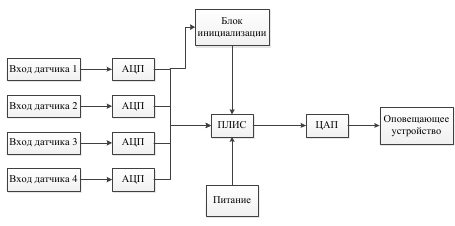
\includegraphics[width=150mm]{src/pictures/offerp1.png}
			\caption{Структурная схема на ПЛИС}\label{offerp1}
		\end{figure}
		\begin{figure}[ht!]
			\centering
			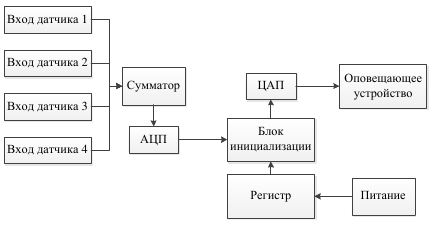
\includegraphics[width=150mm]{src/pictures/offerp2.png}
			\caption{Структурная схема на компараторе и микроконтроллере}\label{offerp2}
		\end{figure}

		Сравнение вариантов реализации представлено в таблице \ref{offert1}.
		\begin{longtable}[t]{@{\extracolsep{\fill}}|l|@{\hskip-14pt}p{0.3\textwidth}|@{\hskip-14pt}p{0.3\textwidth}|}
	\caption{Сравнение реализаций} \label{offert1} \\ \hline
	Вид & На ПЛИС & На регистре и компораторе \\ \hline
	\endfirsthead
	\caption* {Продолжение таблицы \ref{offert1}}\\ \hline
	Вид & На ПЛИС & На регистре и компораторе \\ \hline
	\endhead
	Структура	&
		1) ПЛИС хранит установленные настройки и суммирует значения датчиков. 

		2) Сравнение установленных настроек и показателей датчиков производится посредством ПЛИС. 

		3) Результат сравнения преобразуется из цифрового сигнала в аналоговый.
					&
		1) Цифровой регистр хранит установленные настройки. 

		2) Значения с датчиков проходят через сумматор. 

		3) Сравнение установленных настроек, хранимых в регистре, и показателей датчиков производится с помощью компаратора. 

		4) Выходная информация с компаратора преобразуется в аналоговый сигнал.
		\\ \hline
	Преимущества	&
		Низкое энергопотребление
					&
		Простой ремонт, низкая стоимость
		\\ \hline
	\shortstack{\\ Примерная\\ стоимость}	&
		1750
					&
		1200
		\\ \hline
\end{longtable}


	\section{Выбор датчиков}
		Датчик движения - это устройство для получения информации о состоянии контролируемой им системы, преобразующее данные об изменении характеристик исследуемой области в сигнал, удобный для дальнейшего использования.
		\subsection{Выбор типа датчиков}
			Под понятием «датчик движения» или «датчик присутствия», часто скрываются устройства совершенно разного принципа действия, выполняющие единую задачу, только различными способами.

			В настоящее время наибольшее распространение получили следующие виды датчиков движения:
			\begin{itemize}
\changefontsizes[14pt]{14pt}
				\item Инфракрасные датчики движения (ИК);
				\item Ультразвуковые датчики движения (УЗ);
				\item Микроволновые датчики движения (СВЧ).
			\end{itemize}
			Плюсы и минусы представлены в таблице \ref{offert2}.
			{
\changefontsizes[14pt]{14pt}
\begin{longtable}[t]{@{\extracolsep{\fill}}|l|@{\hskip-14pt}p{0.3\textwidth}|@{\hskip-14pt}p{0.3\textwidth}|}
	\caption{Сравнение видов датчиков} \label{offert2} \\ \hline
	Вид & Преимущества & Недостатки \\ \hline
	\endfirsthead
	\caption* {Продолжение таблицы \ref{offert2}}\\ \hline
	Вид & Преимущества & Недостатки \\ \hline
	\endhead
	Инфракрасные	&
		Возможность довольно точной регулировки дальности и угла обнаружения движущихся объектов

		Удобен в использовании вне помещений т.к. реагирует лишь на объекты имеющие собственную температуру

		При работе абсолютно безопасны для здоровья человека или домашних питомцев, т.к. работает как «приемник», ничего не излучая
					&
		Возможность ложных срабатываний. Из-за того, что датчик реагирует на любые ИК (тепловые) излучения, могут случаться ложные срабатывания даже на теплый воздух, поступающий из кондиционера, радиаторов отопления и т.п.

		Снижена точность работы на улице. Из-за воздействия окружающих факторов, таких как прямой солнечный свет, осадки и т.п.

		Относительно небольшой диапазон рабочих температур

		Не обнаруживает объекты облаченные/покрытые не пропускающими ИК - излучение материалами
		\\ \hline
	Ультразвуковые	&
		Относительно невысокая стоимость

		Не подвергаются влиянию окружающей среды

		Определяют движение вне зависимости от материала объекта

		Имеют высокую работоспособность в условиях высокой влажности или запылённости

		Не зависят от влияния температуры окружающей среды или объектов
					&
		Многие домашние животные слышат ультразвуковые частоты, на которых работает датчик движения, что зачастую вызывает у них сильный дискомфорт

		Относительно невысокая дальность действия

		Срабатывает только на достаточно резкие перемещения, если двигаться совсем плавно – возможно обмануть ультразвуковой датчик движения
		\\ \hline
	Микроволновые	&
		Имеет более высокую стоимость относительно датчиков других типов с аналогичными показателями

		Возможность ложных срабатываний, из-за движений вне необходимой зоны наблюдения, за окном и т.п.

		СВЧ излучение небезопасно для здоровья человека
					&
		Датчик способен обнаруживать объекты за разнообразными диэлектрическими или слабо проводящими ток препятствиями: тонкими стенами, дверьми, стеклами и т.п.

		Работоспособность датчика не зависит от температуры окружающей среды или объектов

		Микроволновый датчик движения способен реагировать на самые незначительные движения объекта

		Датчик обладает более компактными размерами

		Может иметь несколько независимых зон обнаружения
		\\ \hline
\end{longtable}
}

		\subsection{Выбор производителя датчиков}
			Компания «Сибирский Арсенал» - производитель охранных систем, работающий на рынке с 1992 года. Система качества этой компании сертифицирована на соответствие международному стандарту ISO 9001.
			Введу того, что эта компания достаточно компетентна, и их демократичная ценовая политика даёт возможность сделать выбор среди датчиков марки «Рапид».
		\subsection{Выбор датчика марки <<Рапид>>}
			После анализа предложенных вариантов был выбран вариант с ПИД-регулятором, т.к. вариант на ПЛИС имеет более высокую себестоимость.

			Выбор датчика был произведён между датчиками марки «Рапид»: Рапид-3; Рапид-2; Рапид-10. Сравнение вариантов представлено в таблице \ref{offert3}.
			\begin{longtable}[t]{@{\extracolsep{\fill}}|@{\hskip3pt}p{0.3\textwidth}|l|l|l|}
	\caption{Сравнение видов датчиков} \label{offert3} \\ \hline
	Датчик & Рапид-3 & Рапид-2 & Рапид-10 \\ \hline
	\endfirsthead
	\caption* {Продолжение таблицы \ref{offert3}}\\ \hline
	Датчик & Рапид-3 & Рапид-2 & Рапид-10 \\ \hline
	\endhead
	Дальность обнаружения
	человека, не менее		&	15м	&	10м	&	15м	\\ \hline
	Диапазон скоростей
	движения нарушителя		&	0,3-3,0 м\/с	&	0,3-3,0 м\/с	&	0,3-3,0 м\/с	\\ \hline
	Длительность тревожного
		извещения			&	2,5 с	&	2,5 с	&	2 с	\\ \hline
	Диапазон напряжений
		питания от шлейфа
		сигнализации		&	8...30 В	&	3 В	&	9...15 В	\\ \hline
	Вес						&	100 г	&	150 г	&	50 г	\\ \hline
	Потребляемый ток		&	250 мкА	&	-	&	14 мА	\\ \hline
	Диапазон рабочих
		температур			&	-30...+50	&	-10...+50	&	-30...+50	\\ \hline
	Относительная влажность
		воздуха при температуре
		+35 °С, без конденсации 
		влаги, не более		&	95\%	&	95\%	&	95\%	\\ \hline
	Габаритные размеры 		&	90х58х45 мм	&	90х58х45 мм	&	90х58х45 мм	\\ \hline
	Срок службы, не менее	&	10 лет	&	5 лет	&	10 лет	\\ \hline
	Стоимость				&	434	&	1613	&	657	\\ \hline
\end{longtable}

	\section{Заключение по проведённым анализам}
		После анализа предложенных вариантов реализации был выбран вариант c микроконтроллером, т.к. вариант на ПЛИС имеет более высокую себестоимость.

		После анализа предложенных вариантов инфракрасных датчиков был выбран  Рапид-3, т.к. вариант является наиболее экономичным.
